\chapter{Discusión y limitaciones}\label{cap:discusion}

\section{Qué se puede afirmar}

La respuesta del trabajo descansa en la armonía y en la concentración de los cuartos de tono, que son las medidas más
fiables de la herramienta. La armonía acierta el 85\,\% en los compases confiables, incluso en la prueba ciega, y el
método no exagera la novedad: con rock real casi siempre encuentra vecino. La concentración de los cuartos de tono separa
a la banda del control con un margen amplio (48--82\,\% frente a 28--37\,\%), y ese margen es mayor que el error de la
herramienta.

\section{El parecido con el radif es de escala, no de influencia}

El test mide si la distribución de los cuartos de tono de una canción tiene vecinos cercanos entre las piezas del Radif
Corpus. Cuatro de las seis canciones los tienen: Mata Zyklek (percentil 13.5), Yor Zarad (10.9), Utzp (32.3) y Angor
(35.4). Las dos de la familia dórica, Sarniezz (3.9) y Fabienk (0.4), quedan por debajo del umbral de 5. Eso quiere decir
que la banda usa grados fijos en cuarto de tono y que, fuera del modo dórico, los reparte de forma parecida a esa tradición. No prueba que la banda conozca el radif ni que lo
haya tomado como modelo: el mismo reparto podría venir de otra tradición sin corpus simbólico disponible, como el maqam
árabe, o de una elección propia. Para hablar de influencia harían falta fuentes externas.

\section{El bloque de escala en 12 notas no discrimina}

En ese bloque los cuartos de tono se reparten entre los semitonos vecinos y la melodía se compara con corpus de 12 notas.
Las canciones de control de Primus, que no usan cuartos de tono, salen tan típicas como las de la banda («Tommy the Cat»
9.6 y «My Name Is Mud» 6.1 en el radif, frente a 8.7 a 9.6 de la banda). La causa más probable es que las melodías de los
corpus (la voz en el RS~200, una notación de tradición oral en el radif) no son del mismo tipo que la línea aguda que
extrae la herramienta, que en estas grabaciones es sobre todo guitarra y bajo. Los resultados de este bloque se informan,
pero no entran en la conclusión.

\section{El compás cambiante queda sin vecino, no demostrado como nuevo}

Mata Zyklek, Fabienk y Yor Zarad mezclan compases dentro de la misma canción. Ninguna pieza del RS~200 ni del iRealPro,
los dos corpus con compás de la comparación final, hace eso: cada pieza tiene un solo compás. SymbTr, con usules de 7, 9 y
10 tiempos pero también uno solo por pieza, se revisó y no entró en la comparación final. Por eso el resultado dice que no
hay antecedente en los corpus revisados, no que no lo haya en ninguna música. El estilo más cercano en la literatura es
el rock progresivo y el math rock, y el corpus que permitiría comprobarlo (ProgGP) no estuvo disponible.

\section{Comparación con los repertorios}\label{sec:repertorios}

Además de los corpus, el mismo cuaderno se corrió sobre canciones de los artistas que la banda o los analistas mencionan:
King Gizzard (9 temas de \emph{Flying Microtonal Banana}), Frank Zappa (6), King Crimson (6) y Gentle Giant (6), junto con
los tres controles de Primus. En total son 36 canciones medidas con los mismos parámetros. La
tabla~\ref{tab:repertorios} resume las tres medidas que distinguen a la banda y el veredicto del test por bloques.
Las métricas crudas de las 36 canciones, artista por artista, están en el apéndice (figuras~\ref{fig:tarjetas1}
y~\ref{fig:tarjetas2}).

\begin{table}[ht]
  \centering\small
  \caption{La banda frente a los repertorios comparados. \cuarto{} de tono: porcentaje medio de la melodía en cuartos de
  tono (rango entre paréntesis). Concentración: porcentaje de los cuartos de tono en los dos grados más usados. $R$: media
  del mejor periodo de repetición. «Existente»: canciones con veredicto «estilo existente».}\label{tab:repertorios}
  \begin{tabular}{@{}lrlllr@{}}
    \toprule
    Grupo & Temas & \cuarto{} de tono & Concentración & $R$ medio & Existente \\
    \midrule
    Angine de Poitrine & 6 & 16.1 (5.0--25.3) & 48--82 & 0.83 & 0 de 6 \\
    King Gizzard & 9 & 9.9 (3.4--28.0) & 59--100 & 0.69 & 4 de 9 \\
    King Crimson & 6 & 8.8 (0.1--25.0) & 37--82 & 0.52 & 1 de 6 \\
    Gentle Giant & 6 & 2.9 (0.9--6.4) & 38--87 & 0.51 & 0 de 6 \\
    Frank Zappa & 6 & 4.1 (1.6--7.0) & 31--54 & 0.45 & 3 de 6 \\
    Primus (control) & 3 & 11.3 (9.1--13.0) & 28--37 & 0.44 & 2 de 3 \\
    \bottomrule
  \end{tabular}
\end{table}

Tres observaciones matizan la conclusión.

\paragraph{La concentración solo se interpreta por encima del piso de ruido.} Gentle Giant y King Crimson tienen
concentraciones altas (hasta 87\,\% en «Playing the Game» y 82\,\% en «Discipline») con muy poco tiempo en cuartos de tono
(1.0 y 0.1\,\%). Ahí la concentración describe unos pocos errores de medición, no una escala. En Zappa y Gentle Giant el
tiempo en cuartos de tono queda incluso por debajo del de Primus. Lo que distingue a la banda es tener a la vez mucho tiempo
en cuartos de tono, por encima del piso de ruido, y concentrado en pocos grados; por eso el test por bloques solo cuenta la concentración cuando hay al menos 10~s de
melodía en cuarto de tono. El perfil de la figura~\ref{fig:perfil}
lo muestra frente a Primus y King Gizzard: en cuartos de tono en la melodía, la banda tiene la mediana más alta y King
Gizzard la dispersión más amplia, mientras que Primus, sin cuartos de tono reales, se queda en el piso de ruido.

\begin{figure}[htbp]
  \centering
  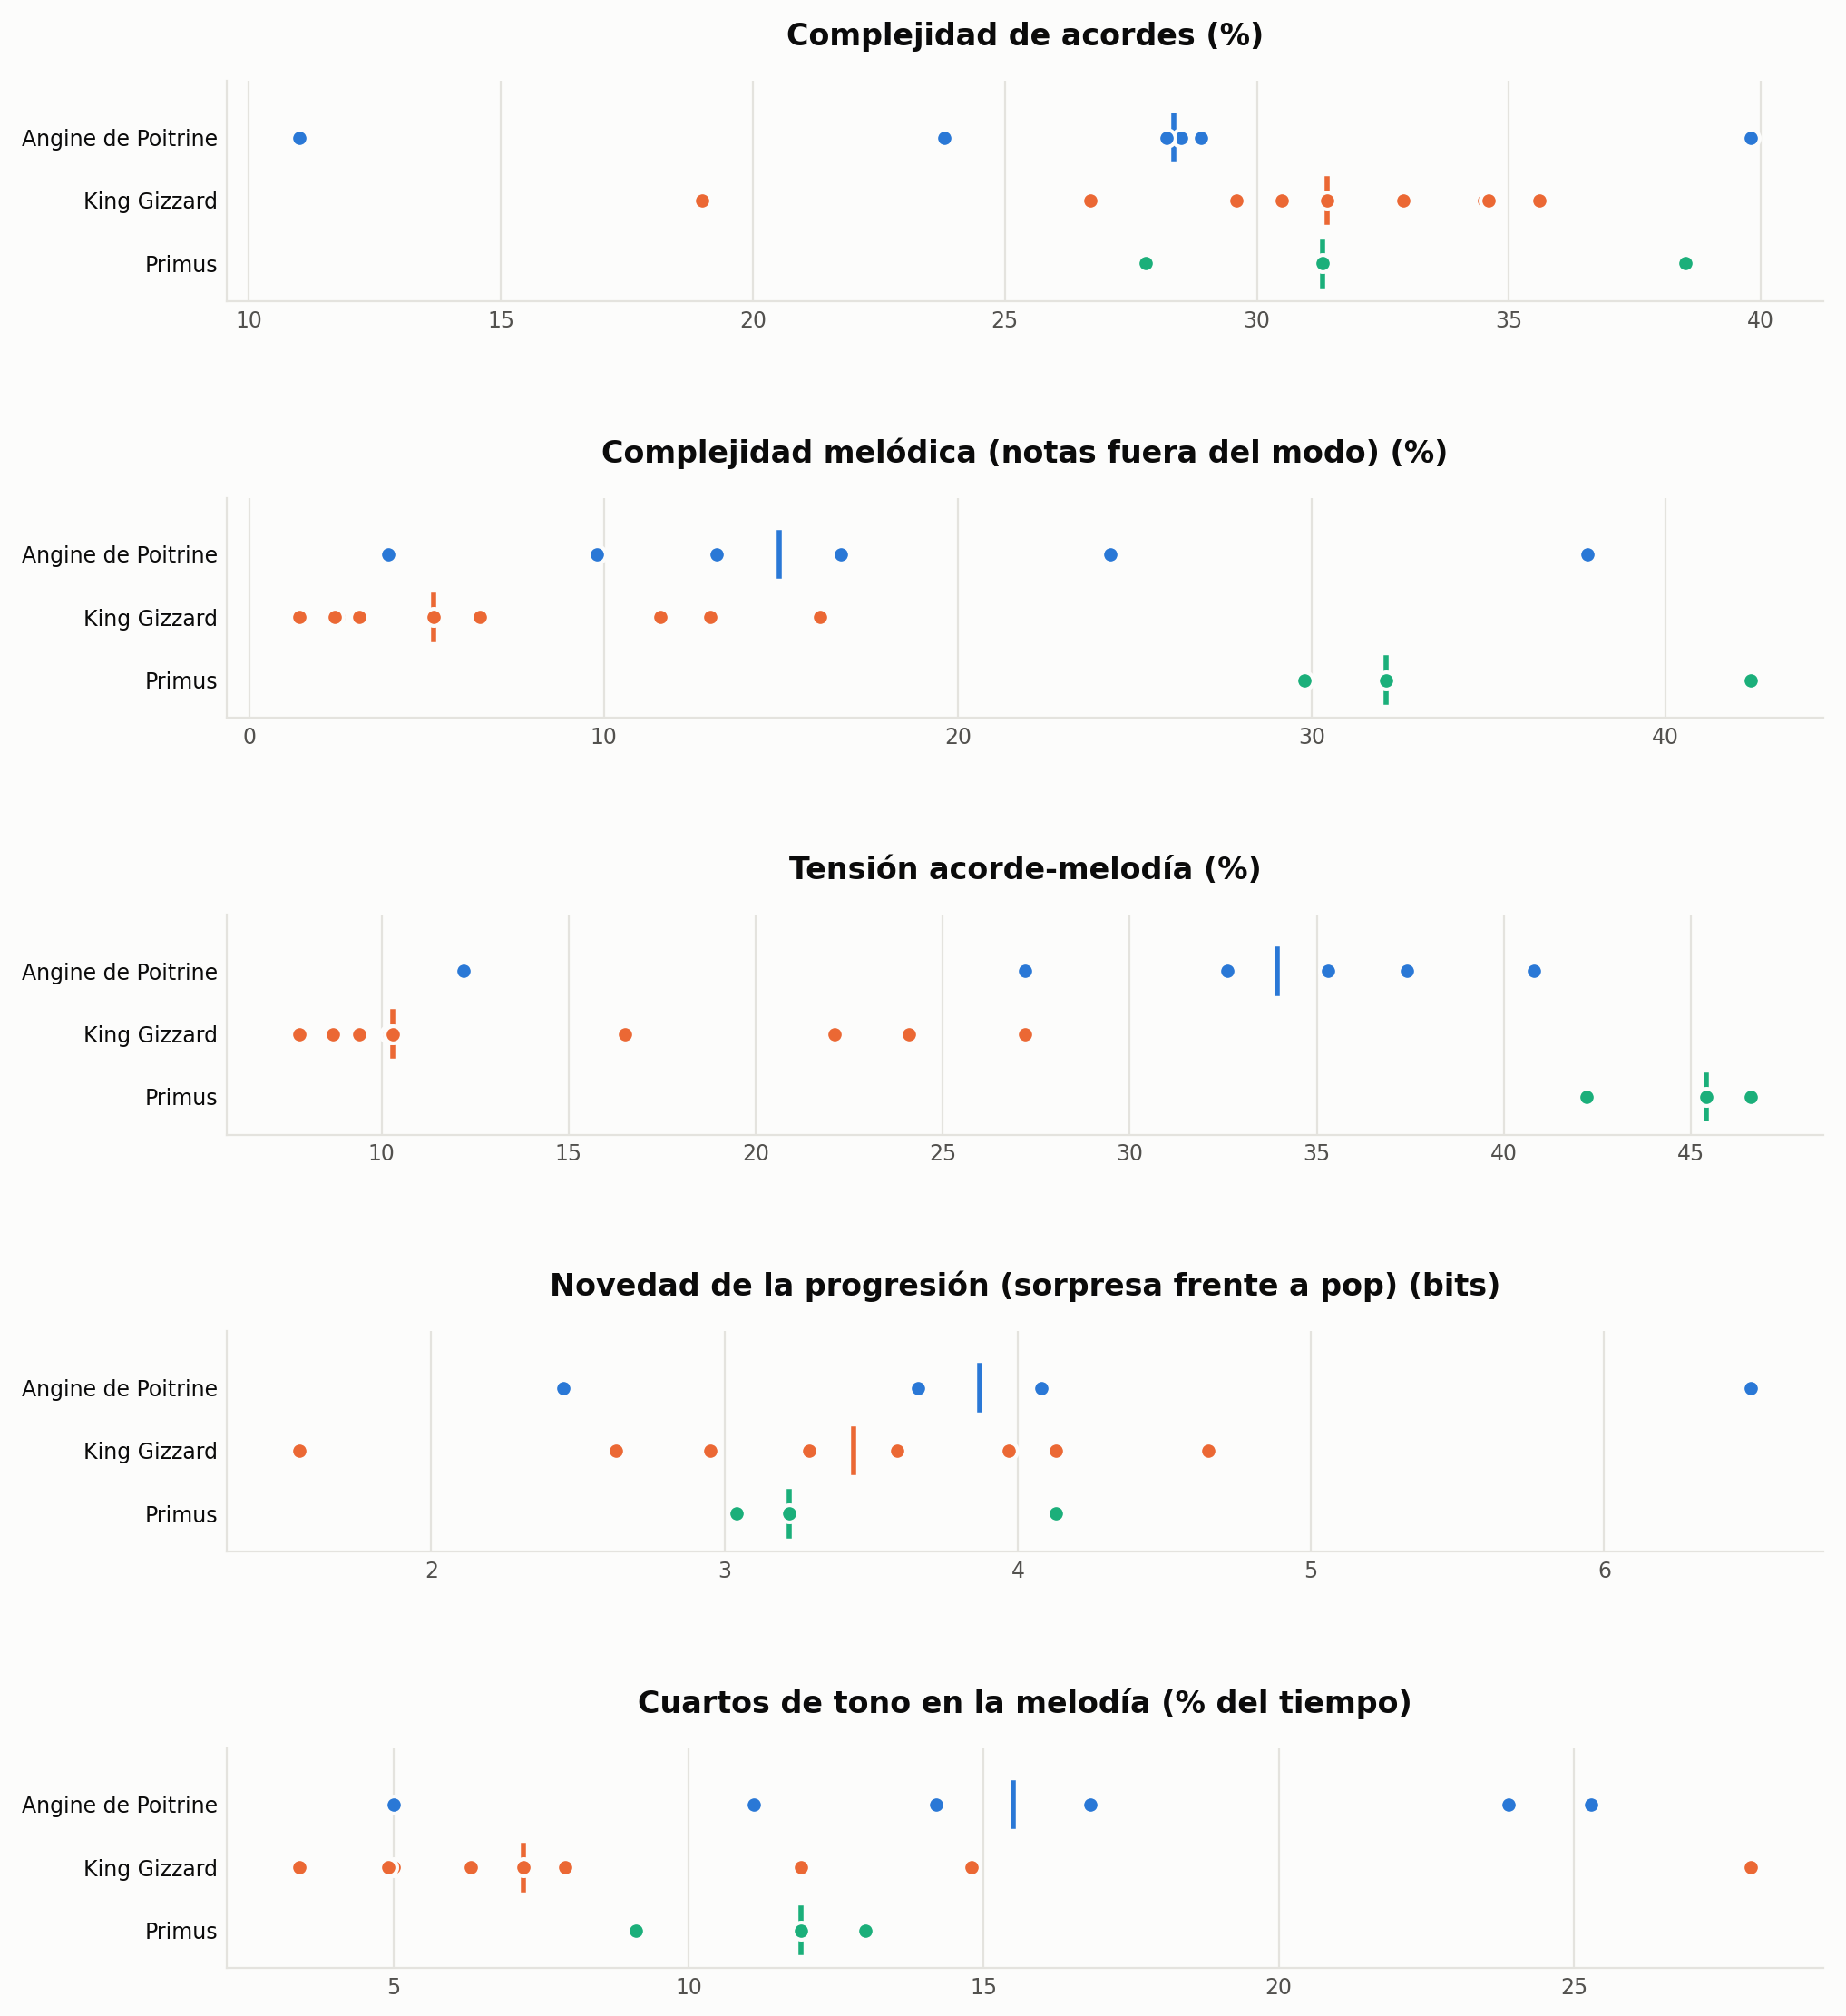
\includegraphics[width=0.85\textwidth]{g_perfil.png}
  \caption{Perfil estructural: la banda (azul) frente a Primus (verde, control) y King Gizzard (naranja). Cada punto es una canción; la raya vertical, la mediana del grupo.}\label{fig:perfil}
\end{figure}

\paragraph{King Gizzard es el vecino más cercano, y comparte dos de los tres rasgos.} Es el único repertorio con cuartos
de tono reales y concentrados (por ejemplo «Doom City», con 28\,\% y 95\,\%) y con ciclos casi tan estables ($R$ medio de
0.69, frente a 0.83 de la banda y 0.44--0.52 del rock progresivo). Su familia de cuartos de tono es la frigia
(\fl2+ y \fl6+ son sus dos grados principales en 5 de sus 9 temas;
«Doom City» combina \fl2+ con 7+). Lo que King Gizzard no tiene es la familia dórica de Sarniezz y Fabienk, y casi la
mitad de sus temas (4 de 9) sí reciben el veredicto «estilo existente (rock)». La figura~\ref{fig:comparar-kg} mide la
distancia de cada canción de la banda a cada tema de King Gizzard y de Zappa, primero solo en los grados en cuarto de tono
y luego en conjunto, con los tres temas de Primus como referencia.

\begin{figure}[htbp]
  \centering
  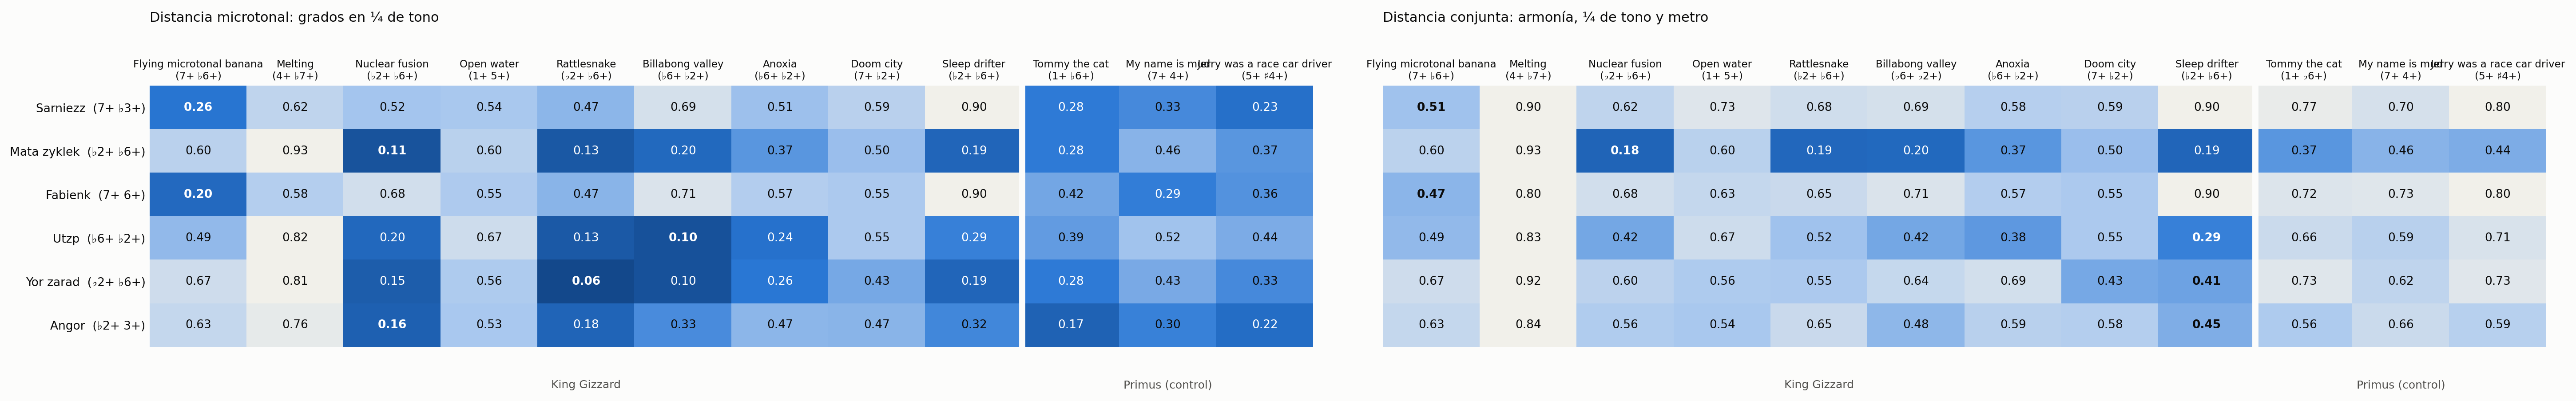
\includegraphics[width=\textwidth]{g_comparar_kg.png}\\[1em]
  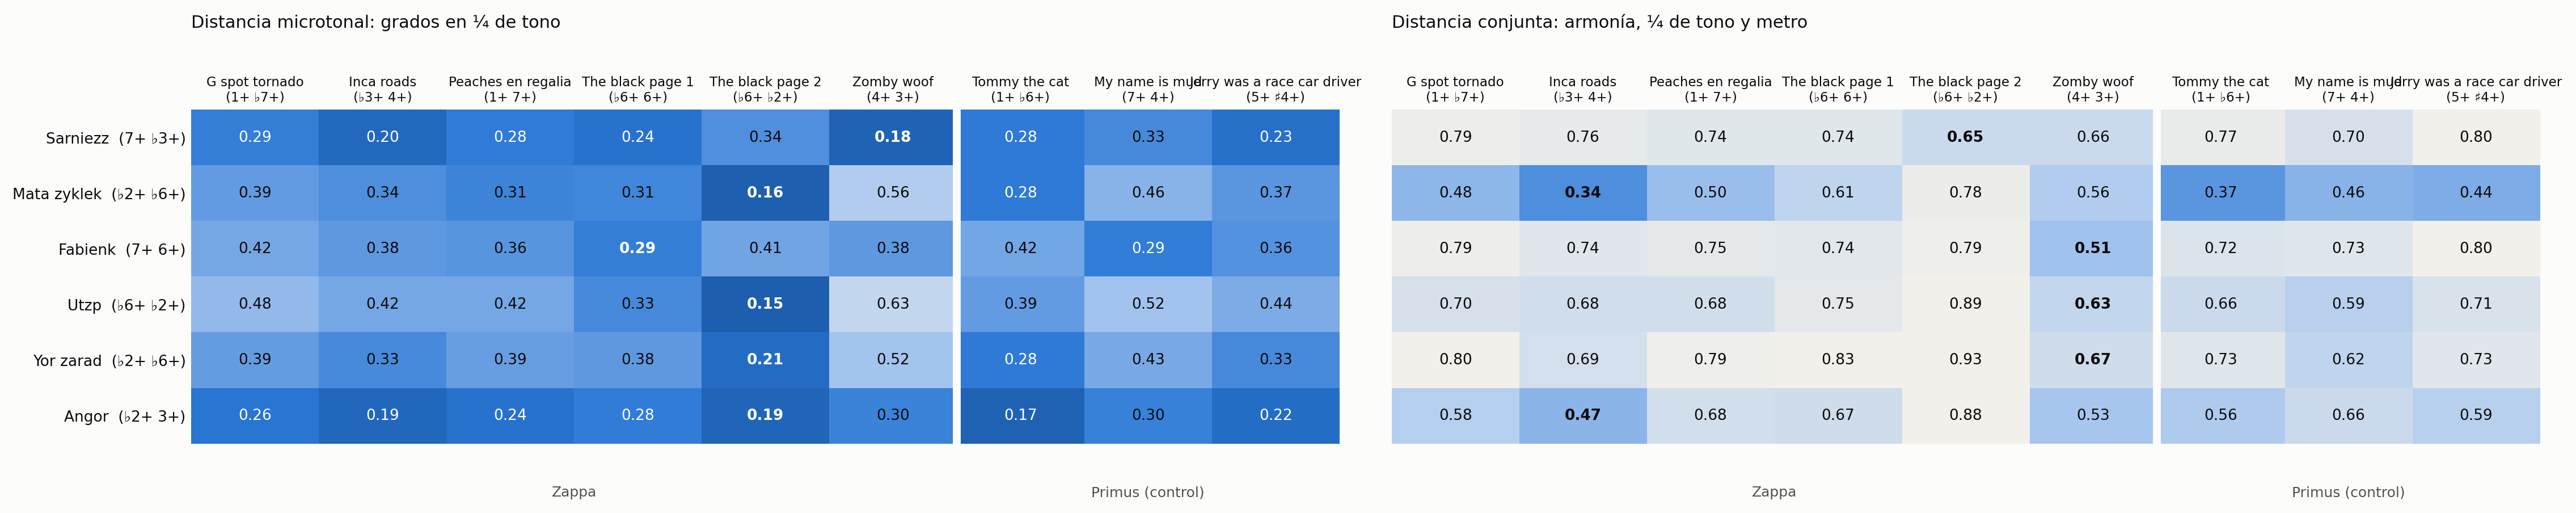
\includegraphics[width=\textwidth]{g_comparar_zappa.png}
  \caption{Distancia de Jensen-Shannon de cada canción de la banda (filas, con sus dos grados en cuarto de tono más usados) a King Gizzard (arriba) y Zappa (abajo), con Primus como control. Izquierda: solo cuartos de tono; derecha: armonía, cuartos de tono y metro. 0 = iguales; más oscuro = más cerca. Bajo cada tema, sus dos grados en cuarto de tono más usados; en negrita, el tema más cercano a cada canción.}\label{fig:comparar-kg}
\end{figure}

\paragraph{El rock progresivo tampoco es un «estilo existente» para estos corpus.} Ninguna canción de Gentle Giant recibe el
veredicto «estilo existente»: todas quedan sin vecino en metro o en armonía, por la misma razón que la banda, que es que
los corpus con compás no tienen piezas con compás cambiante. Por eso el veredicto «sin vecino en metro» no basta, por sí
solo, para afirmar que la banda es nueva: dice que el rock progresivo y el math rock no están representados en los corpus
disponibles. La conclusión del trabajo se apoya, en cambio, en la armonía (fuera de todos los corpus, con la calibración
que lo respalda) y en la melodía (cuartos de tono fijos por encima del piso de ruido, con una familia que ningún corpus ni
repertorio tiene).

Los ciclos de los repertorios refuerzan esta lectura. Las canciones de Zappa, King Crimson y Gentle Giant tienen periodos
variados (de 6 a 32 corcheas, con picos en 5 y en 7 en «The Black Page», «Fracture», «Frame by Frame» y «Level Five»), pero
mucho menos estables que los de la banda: el compás irregular es común en el rock progresivo; la repetición casi idéntica
del looper, no. La figura~\ref{fig:comparar-gg} da las mismas distancias frente a King Crimson y Gentle Giant.

\begin{figure}[htbp]
  \centering
  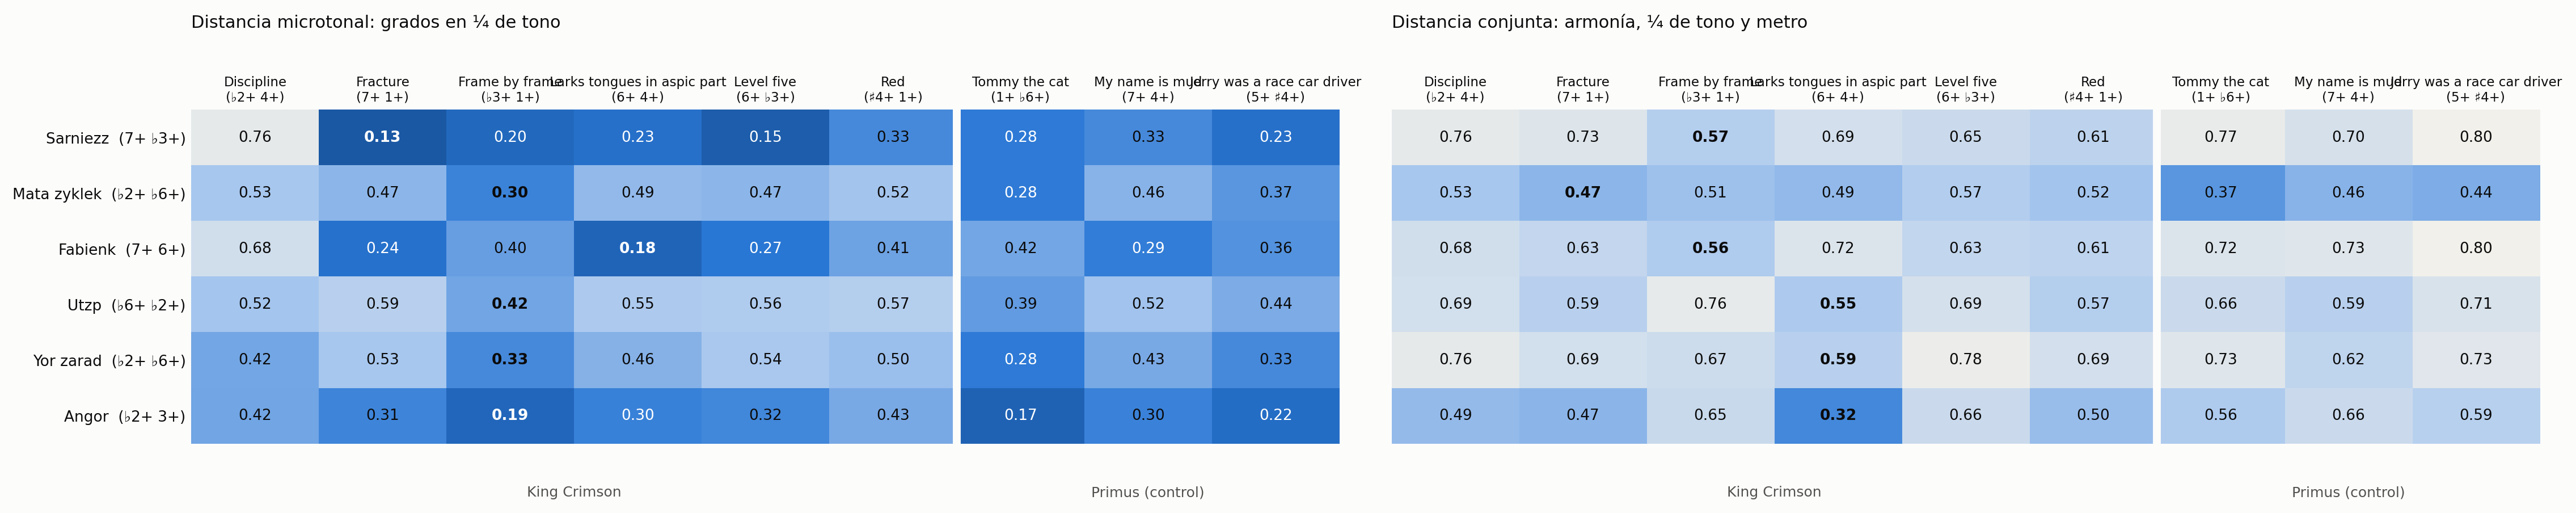
\includegraphics[width=\textwidth]{g_comparar_kc.png}\\[1em]
  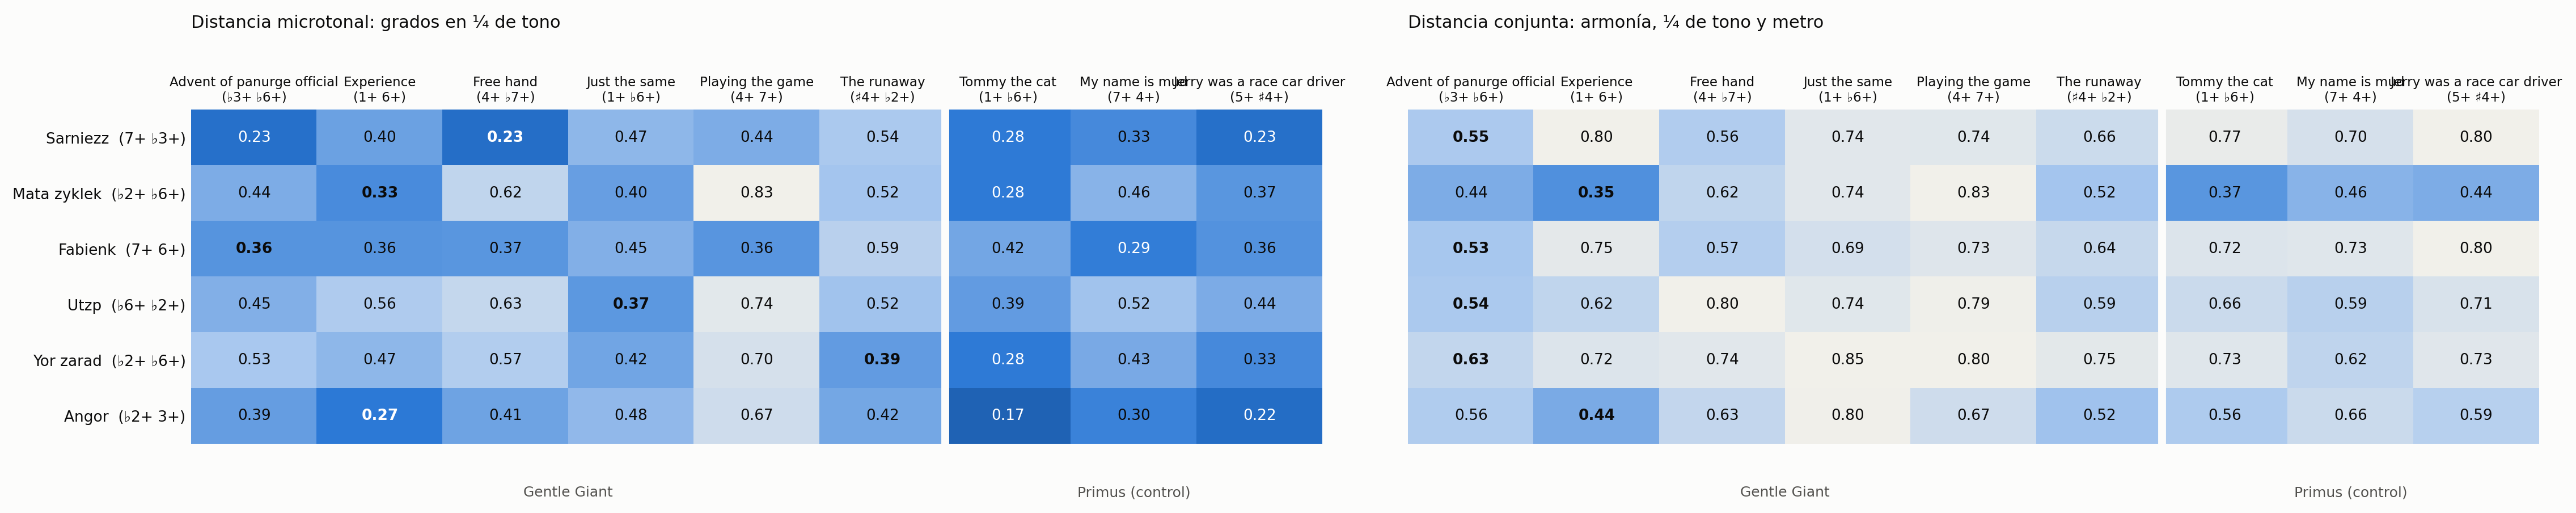
\includegraphics[width=\textwidth]{g_comparar_gg.png}
  \caption{Las mismas distancias frente a King Crimson (arriba) y Gentle Giant (abajo); misma lectura que la figura~\ref{fig:comparar-kg}.}\label{fig:comparar-gg}
\end{figure}

\section{¿Es 24-EDO la rejilla adecuada?}

Todo el análisis supone que la banda toca en 24-EDO, porque así están construidos sus instrumentos. Conviene comprobar que
otra rejilla no describiría mejor lo que suena. La tabla~\ref{tab:edos} lleva los grados que usa el disco a otros
sistemas de afinación y mide cuánto se desafinan.
La figura~\ref{fig:edos} lo muestra grado por grado.

\begin{figure}[htbp]
  \centering
  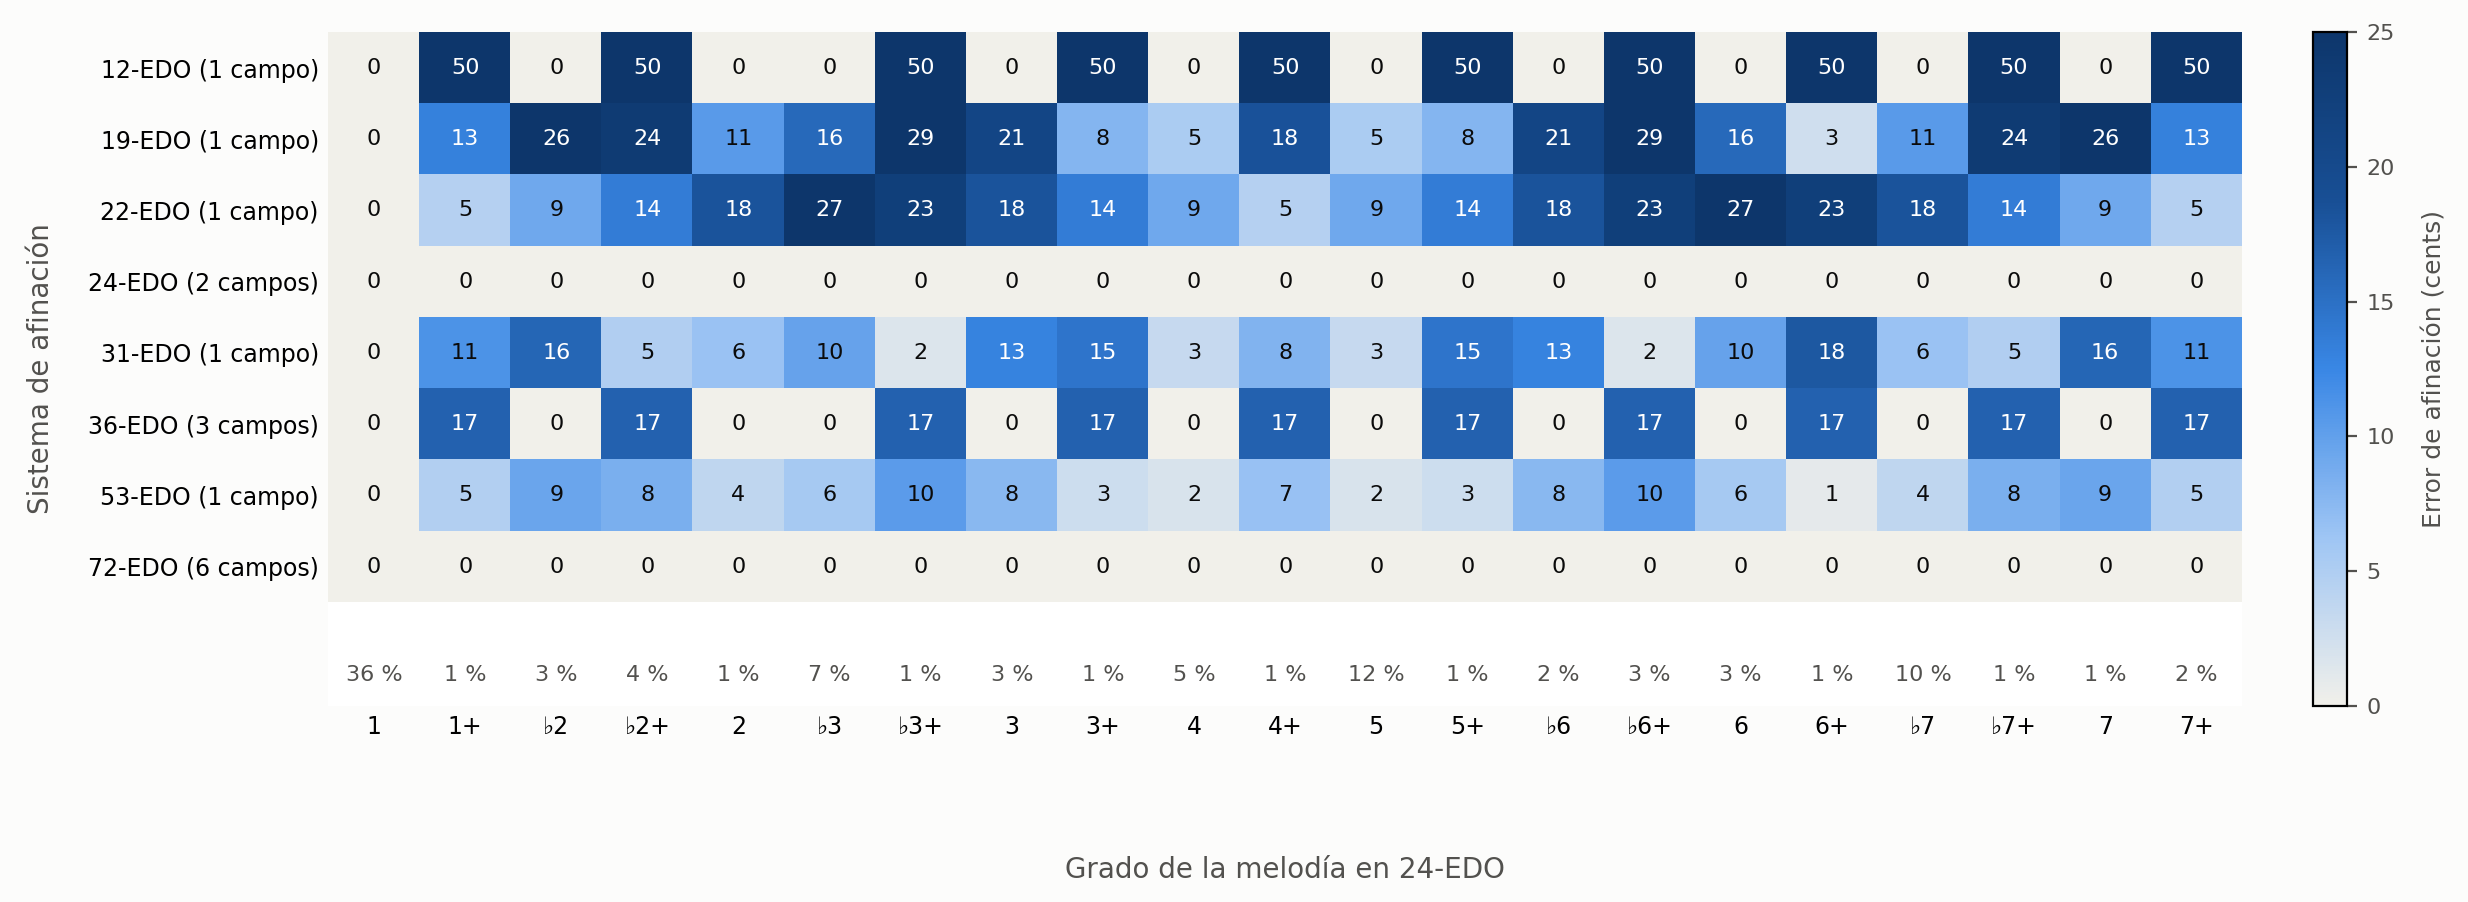
\includegraphics[width=\textwidth]{g_equivalencias_edo.png}
  \caption{Error al llevar cada grado de la melodía de 24-EDO a otro sistema (cents; blanco = sin error, azul oscuro = 25 o más). Entre paréntesis, los campos de quintas de cada sistema; abajo, el uso de cada grado en el álbum.}\label{fig:edos}
\end{figure}

\begin{table}[ht]
  \centering\small
  \caption{Los grados del disco en otros sistemas: error medio (en cents) de los grados usados y de los grados en cuarto
  de tono, y número de campos de quintas.}\label{tab:edos}
  \begin{tabular}{@{}lrrrrl@{}}
    \toprule
    Sistema & Paso & Campos & Error de los grados & Error de los \cuarto & Grados \cuarto{} que se funden \\
    \midrule
    12-EDO & 100.0 & 1 & 8.0 & 50.0 & todos \\
    19-EDO & 63.2 & 1 & 8.9 & 19.2 & \fl2+, \fl3+, \fl6+, \fl7+ \\
    22-EDO & 54.5 & 1 & 9.9 & 14.9 & \fl3+, \fl6+ \\
    \textbf{24-EDO} & \textbf{50.0} & \textbf{2} & \textbf{0.0} & \textbf{0.0} & \textbf{ninguno} \\
    31-EDO & 38.7 & 1 & 4.8 & 7.6 & ninguno \\
    36-EDO & 33.3 & 3 & 2.7 & 16.7 & ninguno \\
    53-EDO & 22.6 & 1 & 3.2 & 6.9 & ninguno \\
    72-EDO & 16.7 & 6 & 0.0 & 0.0 & ninguno \\
    \bottomrule
  \end{tabular}
\end{table}

Por construcción, 24-EDO y sus múltiplos (72-EDO) representan sin error lo que mide la herramienta; el resultado
interesante está en los demás. En 19 y 22-EDO varios grados en cuarto de tono se funden con un grado regular: en ambos
desaparece \fl6+, y con él la familia frigia (\fl2+, \fl6+). En 31 y 53-EDO los grados sobreviven, con errores medios de 3 a 8 cents, pero esos sistemas
tienen un solo campo de quintas: la separación entre la armonía, en el campo regular, y los grados de la melodía, en el
otro campo, deja de existir, y con ella el «desplazamiento de campos» de la sección~\ref{sec:res-haba}. 24-EDO es, entonces,
el sistema más pequeño que conserva a la vez los grados que usa la banda y la estructura de dos campos que organiza su
música.

La escala de la melodía del disco, tomando la variante más usada de cada grado móvil, es 1 · \fl2+ · \fl3 · 4 · 5 · 6 ·
\fl7: un dórico con la segunda neutra. Las fundamentales quedan en el campo regular y la melodía usa sus grados en cuarto de
tono en el otro campo.

\section{Modos compartidos con King Gizzard}

El modo de cada canción, descrito por los grados 2, 3, 6 y 7, permite una comparación más fina que el reparto de grados.
Utzp (\fl2+, \fl3, \fl6+, \fl7) tiene exactamente el mismo modo que «Nuclear Fusion», «Sleep Drifter» y «Billabong
Valley» de King Gizzard; «Rattlesnake» y «Doom City» comparten la segunda neutra \fl2+ sobre un frigio. Ninguna canción de
King Gizzard tiene el modo de Mata Zyklek y Yor Zarad (\fl2+, 3, \fl6+, \fl7), con tercera mayor, ni el dórico con
cuartos de tono en la melodía de Fabienk y Sarniezz. El parentesco con King Gizzard es, por tanto, real pero parcial: comparten
la familia frigia, no las otras dos.

\section{Límites de la herramienta}

\begin{itemize}
  \item \textbf{Melodía.} La melodía acierta entre el 37 y el 66\,\% según la canción. El cuello de botella es separar las
  capas del looper: en muchos cuadros la melodía no aparece entre los picos de la saliencia, y ni la estructura del
  looper, ni el estéreo, ni un separador mejor la destapan.
  \item \textbf{Armonía de Sarniezz.} Acierta el 58\,\%, por su riff cromático de cuartos de tono, su acorde sus2 y su bajo
  un cuarto de tono bajo.
  \item \textbf{Centro tonal fuera de la banda.} La elección del centro falla en algunas canciones ajenas: «Tommy the Cat»
  sale en Sol en vez de Mi.
  \item \textbf{Pocas canciones.} El álbum tiene seis canciones y solo cuatro tienen referencia.
  \item \textbf{Corpus.} Ningún corpus de armonía tiene cuartos de tono, y los corpus microtonales simbólicos no
  representan necesariamente la afinación real de una interpretación. Los corpus de rock y pop tienen sesgos de selección
  y de transcripción.
  \item \textbf{Separación.} La comparación entre separadores se hizo en una sola canción; no basta para generalizar.
\end{itemize}

\section{Primus y las influencias}

La comparación con Primus muestra parecidos puntuales: «Tommy the Cat» comparte con Fabienk y Sarniezz el centro (Mi, el de la
partitura, aunque la herramienta lo elija mal), el modo dórico y las fundamentales 1, \fl3 y \fl7, y «My Name Is Mud» es un pedal, como Mata Zyklek. Pero Primus no tiene ciclos
de looper ni cuartos de tono concentrados, y cambia más de acorde. Como ninguna fuente pública lo cita como influencia, se
presenta solo como comparación propia. Del mismo modo, King Gizzard es el vecino más cercano en conjunto, pero la banda no
lo cita; lo propone un analista.
